\section{Introduction}
As discussed in previous chapters, the proposed software solution takes the form of two mobile phone applications. This chapter describes and outlines the requirements for our software solution. Requirements will set goals for the functionality of the software, whereas the design section allows us to translate these requirements onto paper. Both sections will become useful when testing whether the system is fit-for-purpose.

\section{Requirement Engineering}
One of the most important activities in software engineering is to specify the software. In this section, system requirements will be presented. Two sources of requirements were used: firstly using information discovered from the literature and technology survey; and secondly from an interview with a project manager at `Company A'\footnote{Company A is a large multinational organisation employing over 100,000 people across 168 countries}. These requirements are not to be used as an exhaustive list, but are to be used as a benchmark for ensuring the created product is fit-for-purpose.

\subsection{The Interview}
To gather business oriented requirements, an interview was conducted with a project manager, specialising in IT implementations for corporate facilities in Company A. Several points discussed were integrated into the system as requirements. The full transcript of the interview can be found in the appendix A. For instance:


{\fontfamily{ppl}\selectfont
Q6. What do you think of this solution? [The corporate loyalty app]

A. For this solution to be feasible and useful, it would need to be:

\begin{itemize}
\item Available for all of our permanent staff to use
\item Easy integration for further sites and users globally
\item Good usability aspects. Company A has 100,000 staff members with a variety of demographics, therefore all users should find it easy to use and better than the existing process
\item The system would need to increment on a daily basis when the staff members enter site (once a day only)
\end{itemize}
}

Informed requirements M2, S2, S4, and C6 (explained in the next section).

\clearpage{}

\subsection{Requirements}
Our solution involves the creation of two Android applications, thus the requirements below will be marked whether they are for \textbf{Both} or exclusively for the \textbf{Loyalty Manager}, or \textbf{Loyalty Stampbook}. Effort will be made to maximise requirements that encompass both applications.  

We found that there was an abundance of potential system requirements, however not all can be implemented in good time. For this reason, we present these requirements in MoSCoW prioritisation format~\cite{brennan2009guide} (Must Have, Should Have, Could Have, Won't Have) in order to categorise the importance of their delivery.

\subsubsection{Must Have}
`Must have' requirements are the minimum amount of features to be satisfied for the success of the system. As a result, these are of highest priority. Requirements defining gamification are not listed here as they are not `key' to the system.
\begin{description}[leftmargin=!,labelwidth=\widthof{\bfseries Medium}]
    \item[M1] \textbf{Sign-In \& Registration} \newline
        \textit{The user should be able to sign in with an existing account or register for a new one} \newline
        [Both Systems] | Functional
        
    \item[M2] \textbf{Fast Stamping} \newline
        \textit{Access to the NFC stamping functionality should be available within a single tap from a home page} \newline
        [Both Systems] | Functional
    
    \item[M3] \textbf{NFC Transmission} \newline
        \textit{The system must use NFC for data transmission and Host Card Emulation} \newline
        [Both Systems] | Functional
        
    \item[M4] \textbf{Online Syncing} \newline
        \textit{The system must be able to sync a users `stampbook' online} \newline
        [Both Systems] | Functional
        
    \item[M5] \textbf{Sync on Interaction} \newline
        \textit{Syncing must take place as soon as there is an interaction that affects the stamp count of a scheme} \newline
        [Both Systems] | Functional
        
    \item[M6] \textbf{Syncing Time} \newline
        \textit{The response time for syncing must be within 5 seconds} \newline
        [Both Systems] | Non-functional  
        
    \item[M7] \textbf{Feedback on Interaction} \newline
        \textit{The system must provide audio/visual feedback whenever a `stamp' has taken place} \newline
        [Both Systems] | Functional
        
\end{description}

\subsubsection{Should Have}
The "should have's" represent features which should be included if the system if time permits. Generally these requirements add a layer of usability and engagement to the system; as such, most of the gamification implementation is defined here.
\begin{description}[leftmargin=!,labelwidth=\widthof{\bfseries Medium}]
    \item[S1] \textbf{Consistency} \newline
        \textit{The system should fit within the standards and design language of the Android operating system} \newline
        [Both Systems] | Non-functional
        
    \item[S2] \textbf{Rewards Browsing} \newline
        \textit{The user should be able to easily browse their rewards available} \newline
        [Loyalty Stampbook] | Functional

    \item[S3] \textbf{Badges} \newline
        \textit{Users should be able to collect badges upon completing certain goals} \newline
        [Loyalty Stampbook] | Functional

    \item[S4] \textbf{Secure Communications} \newline
        \textit{NFC Communications between devices should be encrypted} \newline
        [Both Systems] | Functional

    \item[S5] \textbf{Level-Restrictions} \newline
        \textit{Rewards should have a minimum-level required in order to claim} \newline
        [Loyalty Stampbook] | Functional

    \item[S6] \textbf{Levelling System} \newline
        \textit{Users should be able to level up each of their loyalty schemes independently (20 - gold, 50, platinum)} \newline
        [Loyalty Stampbook] | Functional
        
\end{description}

\subsubsection{Could Have}
These requirements represent bells-and-whistles requirements. Features in the `could have' are desirable but not a necessity to the project's initial builds. Incorporations of these requirements into future builds of the system would greatly benefit user experience.

\begin{description}[leftmargin=!,labelwidth=\widthof{\bfseries Medium}]
    \item[C1] \textbf{Passive Card Emulation} \newline
        \textit{The system could allow passive host card emulation} \newline
        [Loyalty Stampbook] | Functional

    \item[C2] \textbf{Branding} \newline
        \textit{The system could provide deep customisation options for each scheme} \newline
        [Loyalty Manager] | Functional

    \item[C3] \textbf{Internet-Free Stamping} \newline
        \textit{Users could have the ability to gather stamps without being connected to the internet (facilitated by the Manager)} \newline
        [Loyalty Manager] | Functional
        
    \item[C4] \textbf{Multiple Device Support} \newline
        \textit{Users could be able to login and use multiple devices seamlessly} \newline
        [Loyalty Stampbook] | Functional
        
    \item[C5] \textbf{Personalisation} \newline
        \textit{The system could allow users to customise the appearance of their profile} \newline
        [Loyalty Stampbook] | Functional
        
    \item[C6] \textbf{Restricted Schemes} \newline
        \textit{The system could allow for account-specific schemes (only authorised users have access to the scheme)} \newline
        [Both Systems] | Functional
        
    \item[C7] \textbf{Transaction History} \newline
        \textit{The system could have a transaction history to allow users to see their recent activity} \newline
        [Loyalty Stampbook] | Functional
\end{description}

\subsubsection{Won't Have}
`Won't have' requirements are simply outside the scope of the project. Their functionality is either not the purpose of the system (W1), or facilitate unwanted features into the ecosystem (W2).
\begin{description}[leftmargin=!,labelwidth=\widthof{\bfseries Medium}]
    \item[W1] \textbf{Payment Options} \newline
        \textit{The system will not facilitate any form of payment} \newline
        [Both Systems] | Functional  
        
    \item[W2] \textbf{Loyalty Sharing} \newline
        \textit{Users will not be able to transfer stamps between friends/accounts} \newline
        [Loyalty Stampbook] | Functional 
\end{description}

\clearpage{}
\section{Design}
\subsection{Outline}
Turning our attention to the design, here we present the system, matching the requirements, outlining how they meet the system requirements. Some interesting scenarios have been mentioned in the requirements that leave a wide scope of design challenges. A study is also undertaken that involves participatory design as an extension of the proposed design - in effect, asking potential users to tackle these challenges.


\subsection{The Three Components of the System}
\label{sec:databasepls}
As mentioned earlier, the proposed system involves two separate applications. However, in order to meet functional requirements M1, M4, C4 and C6 a database will need to be introduced in order to interconnect user accounts, along with any relevant data (i.e. loyalty schemes, stamps and badges). Furthermore, a database is also useful from a security and continuity standpoint. For instance, backing-up stamps and schemes allows users to sync their accounts between phones, as well as preventing the system from abuse of local files.

\subsection{Modeling The Interaction}
The key design challenge of the system is to ensure seamless and correct communications via NFC between each of the three system modules. As outlined in the literature survey, there are several modes that NFC can adopt~\cite{4278549}, each changing the device's role as part of the interaction. In this case, Host Card Emulation (HCE) and NFC Readers can be setup in different configurations to facilitate these communications. Two such configurations were considered - Loyalty Manager using HCE and Loyalty Stampbook using HCE (Fig. \ref{fig:dArches}). The difference between these configurations is small; however they each have distinct implications.

\begin{figure}[H]
 \centering
  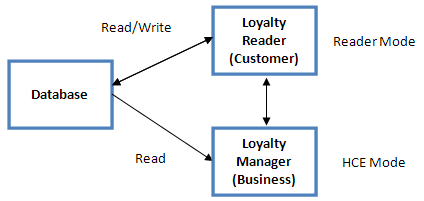
\includegraphics[width=0.48\textwidth]{img/dArch1.png}
   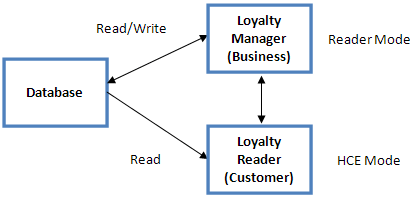
\includegraphics[width=0.48\textwidth]{img/dArch2.png}
    \caption{(i) Loyalty Manager using HCE. (ii) Loyalty Stampbook using HCE}
     \label{fig:dArches}
\end{figure}

\subsubsection{Loyalty Manager using HCE}
Loyalty Manager with HCE entails using the Manager application as a smartcard. In this case, the Loyalty Stampbook interfaces with the database to update the user's Stampbook. 

The benefits (+) and drawbacks (-) of this configuration are: 
\begin{description}[leftmargin=!,labelwidth=\widthof{\bfseries small}]
    \item[+] Syncing is not necessary as the Manager will always have the updated Stampbook
    \item[+] Less logic required in the Applications to direct stamps
    \item[---] Dependant on both applications having internet connection
    \item[---] The user must have the Loyalty Stampbook open to collect stamps
    \item[---] Data integrity issues if people maliciously modify code of the Loyalty Stampbook 
    \item[---] Differentiating between  reward \& stamp requests is difficult
\end{description}
\subsubsection{Loyalty Stampbook using HCE}
When the Loyalty Stampbook acts as the smartcard, several interactions differ. Primarily, the burden of dealing with the database is placed onto the Loyalty Manager.

The benefits (+) and drawbacks (-) of this configuration are: 
\begin{description}[leftmargin=!,labelwidth=\widthof{\bfseries small}]
    \item[+] The Loyalty Stampbook does not need to have the application open to collect a stamp, the phone functions as a passive smartcard.
    \item[+] Only the Loyalty Manager needs access to the internet. Customers will be able to collect and expend stamps whilst not connected
    \item[+] The Loyalty Manager can easily separate stamp requests from reward requests
    \item[+] Data is more secure as only the authorised Loyalty Manager has access to modify the database. Ultimately, this prevents user tampering and ensures data integrity within the system
    \item[---] Complex logic required in both applications
    \item[---] Providing specific feedback directly to the Loyalty Stampbook via the app is difficult
\end{description}

\subsubsection{Chosen Model}
\emph{Loyalty Stampbook using HCE} was selected on the merit of its positives. Primarily, not requiring internet access from the customer, the ability to collect stamps without having the application open and its emphasis on security. On the other hand, it makes the implementation challenging, requiring more logic to support the two-way communications. Nonetheless, we expect that this model will ultimately benefit the system by making it easier to use and understand for users.

\subsubsection{User Feedback}
Requirement M7 identifies the need for user feedback in both applications when stamping. Mobile operating systems provide several design patterns to accommodate interaction feedback, for instance: audio, notifications and haptic/vibration. For the Loyalty Stampbook, notifications were selected as the \textbf{primary} method as users may want to keep their phones on silent. Within the Loyalty Manager, responses can be presented as a simple popup\footnote{`Toasts' are used to achieve this in Android as a form of simple feedback}. Moreover, we integrate an audible sound whenever two NFC devices make contact; however users will be able to mute this feature if the device is placed on silent. 

\subsection{Design Methodology}
In order to develop the designs for the system components, a user-centered design\cite{usercentereddesign} approach was taken for each iteration. The initial wireframe was mocked-up from Android design heuristics as a design language.
\subsubsection{Design Language}
In order to identify the deign language for our system, guidelines to be defined. Usability consultant Jakob Neilson presents ten usability heuristics for interaction design. One such heuristic is `Consistency and Standards'~\cite{jakob}, in this case meaning that the solution should follow the platform conventions and design of our operating system. This satisfies the requirement S1. It is important to highlight that users of our applications are also users of the mobile operating system -- Therefore, if this heuristic is met, users will feel more comfortable with the system as it will feel familiar to use. \emph{Material Design}~\cite{materialDesign}, is a visual design language from the Android OS with a goal to:
\begin{quote}
    \textit{``Develop a single underlying system that allows for a unified [user] experience across platforms and device sizes''}~\cite[Introduction]{materialDesign}
\end{quote}

We present the designs to potential users within our target users (age 16-40). Feedback was captured, analysed and incorporated into the next iteration. In the interest of time, two iterations were incorporated for the Loyalty Stampbook and one for the Loyalty Manager.

\newpage{}
\subsection{Design Process - Loyalty Stampbook}
\subsubsection{Wire-Frame Mockups}
The wire-frames were developed on paper using the Material Design guidelines discussed earlier (Fig. \ref{fig:wireframe1}). An analysis of the design decisions follows: 
\begin{figure}[H]
 \centering
  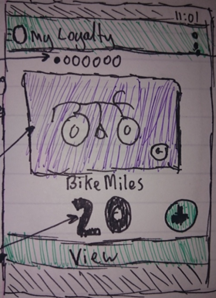
\includegraphics[width=0.26\textwidth]{img/wireframeMockup.png}
    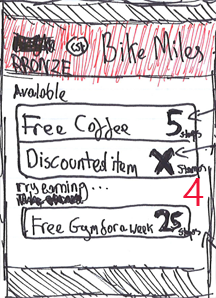
\includegraphics[width=0.26\textwidth]{img/wireframeMockup2.png}
    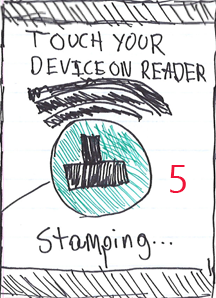
\includegraphics[width=0.26\textwidth]{img/wireframeMockup3.png}
    \caption{The initial wire-frame mockup for the Loyalty Stampbook using the Material Design guidelines}
         \label{fig:wireframe1}
\end{figure}

\begin{enumerate}
  \item `Pips' are a common design pattern on mobile devices. They serve as a page indicator and afford swiping on the screen. In this case, users can see all of their loyalty schemes in this page and can swipe between them. 
  \item The idea of having `loyalty cards' is a metaphor from the real world. Businesses may be able to customise the graphic on the card.  Cards on mobile screens also afford flipping over for more information - within mobile applications this is done via a tap, meaning users can get details of a loyalty scheme by tapping the card.  
  \item Floating Action Buttons (FAB) are special buttons used to present users with the primary action of the application. In this case it is a stamp button that takes users to the stamp screen.
  \item A list of available rewards for the users, notifying them which rewards are available.
  \item A stamp screen to notify the users to tap their device onto the reader. Within this design, all NFC interactions are done with this screen open; however this screen may not be needed using the Loyalty Stampbook using HCE interaction model
\end{enumerate}

\subsubsection{Feedback For Next Iteration}
The design was present to three potential users individually, a list of suggestions follows:
\begin{itemize}
  \item \textit{``If it is so important, shouldn't the stamp button should be in all pages, not just the home page?''}
  \item \textit{``How will gamification work in the design?''}
\end{itemize}

Paper-based mockups are fast and cheap way to prototype a design; however they can make it difficult to communicate links between the actions; Nonetheless, user suggestions were considered for the next iteration.


\subsubsection{Iteration 1 - Mockup}
The first iteration was a near direct translation of the paper wire-frame into a navigable mockup (Fig. \ref{fig:wireframe2}), with a few small changes following previous feedback. A dedicated loyalty scheme page was introduced to track potential gamification concepts (fulfilling requirement S3), along with the addition of a stamp button on every page.
\begin{figure}[H]
 \centering
  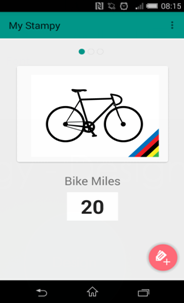
\includegraphics[width=0.29\textwidth]{img/MainMockup.png}
   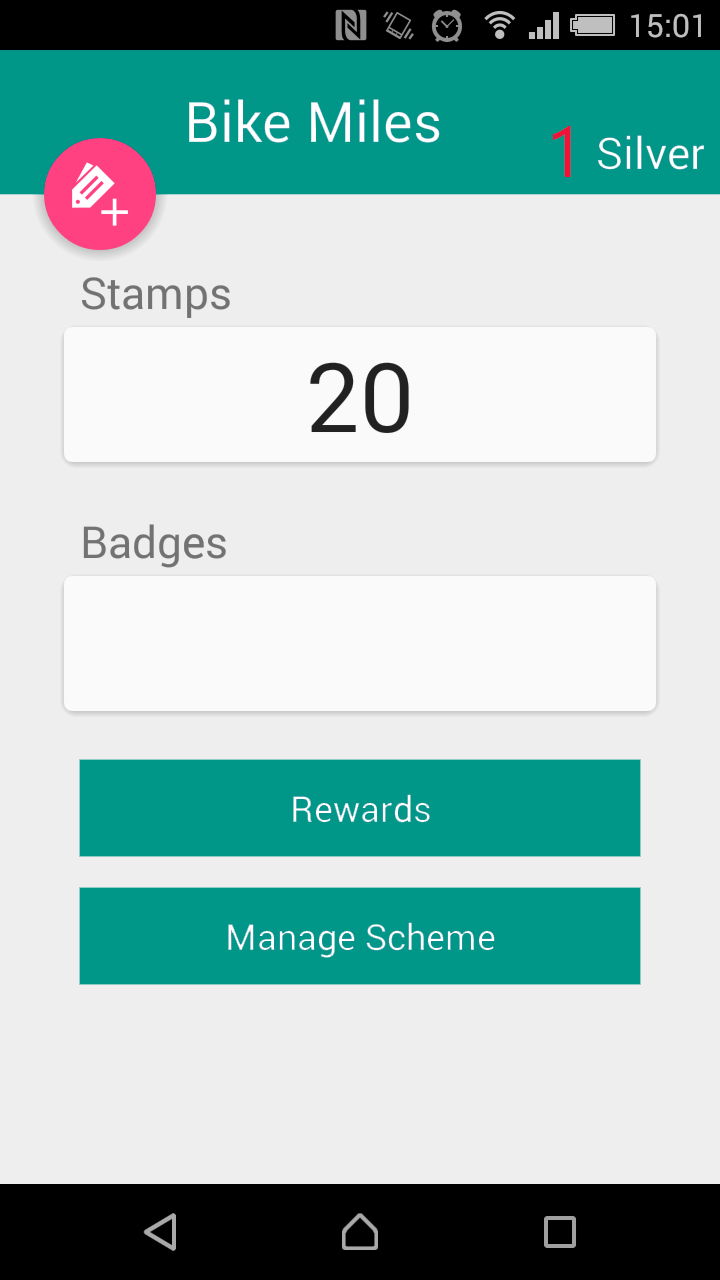
\includegraphics[width=0.27\textwidth]{img/firstiteration1.png}
    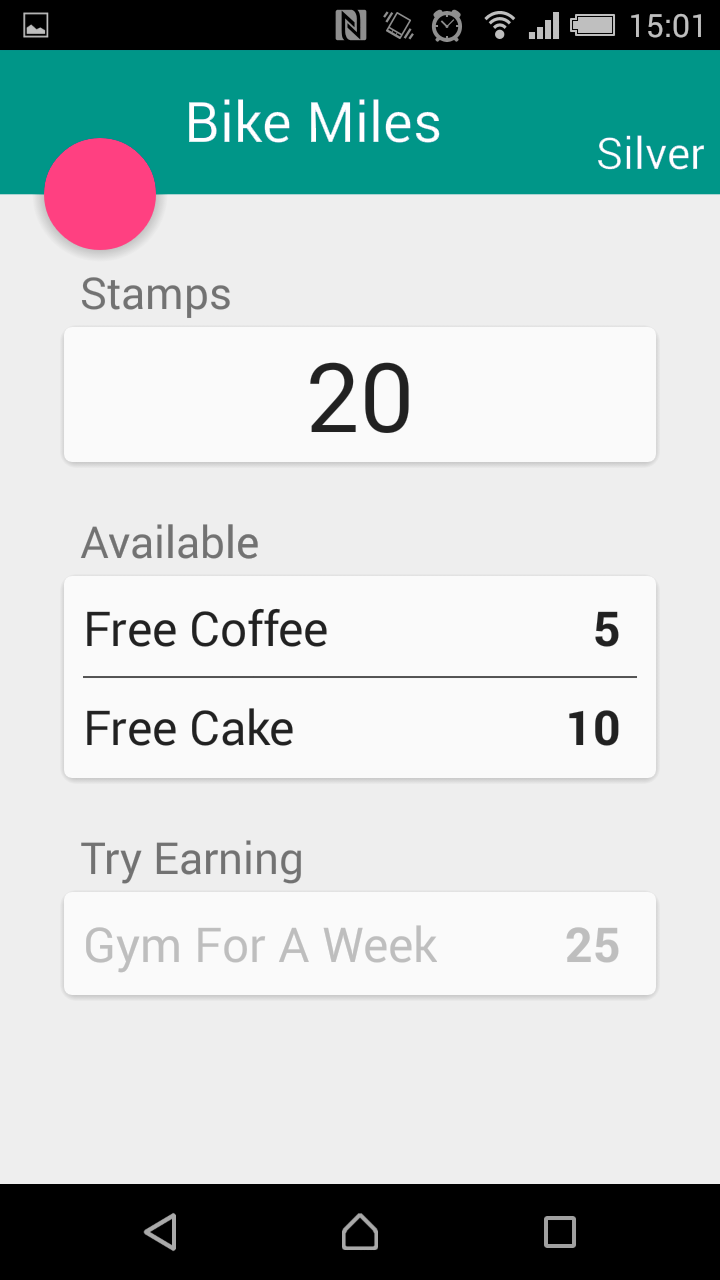
\includegraphics[width=0.27\textwidth]{img/firstiteration2.png}
    \caption{A mockup of the wire-frame incorporating suggestions from last iteration}
	\label{fig:wireframe2}
\end{figure}

\begin{enumerate}
  \item A dedicated loyalty scheme page for the user to explore the current loyalty scheme. These may be customisable for the business. Potential gamification methods, such as levels and badges would live here if implemented.
\end{enumerate}

\subsubsection{Feedback For Next Iteration}
The design was present to three potential users individually, a list of suggestions follows:
\begin{itemize}
  \item \textit{``If I have many loyalty schemes, It feel sluggish to scroll through all of them individually. Perhaps have them as a list''}
  \item \textit{``If I have my own account, there should be a profile page''}
  \item \textit{``It takes too many clicks to get to the rewards''} [2 clicks after finding scheme]
    \item \textit{``The stamp button makes me thing I'm only stamping the visible scheme?''} [This was an unintentional consequence of the design]
     \item \textit{``The app shoulds tell me when I have sufficient stamps to claim a reward''}
\end{itemize}

More issues were identified during this iteration as users were able to explore the design effectively. Nevertheless, feedback clearly suggested that this design was slow, confusing and ultimately - not fit for purpose. Substantial changes had to be made.

\subsubsection{Iteration 2 - Final Design}
In order to remediate some of the design problems identified with the previous feedback, a very different approach had to be taken with the design - as presented in Fig. \ref{fig:wireframe3}. In order to present clarity, several user interface aspects had to be removed; for instance the stamp button was removed and is to be replaced with instructions on how to stamp upon logging-in for the first time.

\begin{figure}[H]
 \centering
  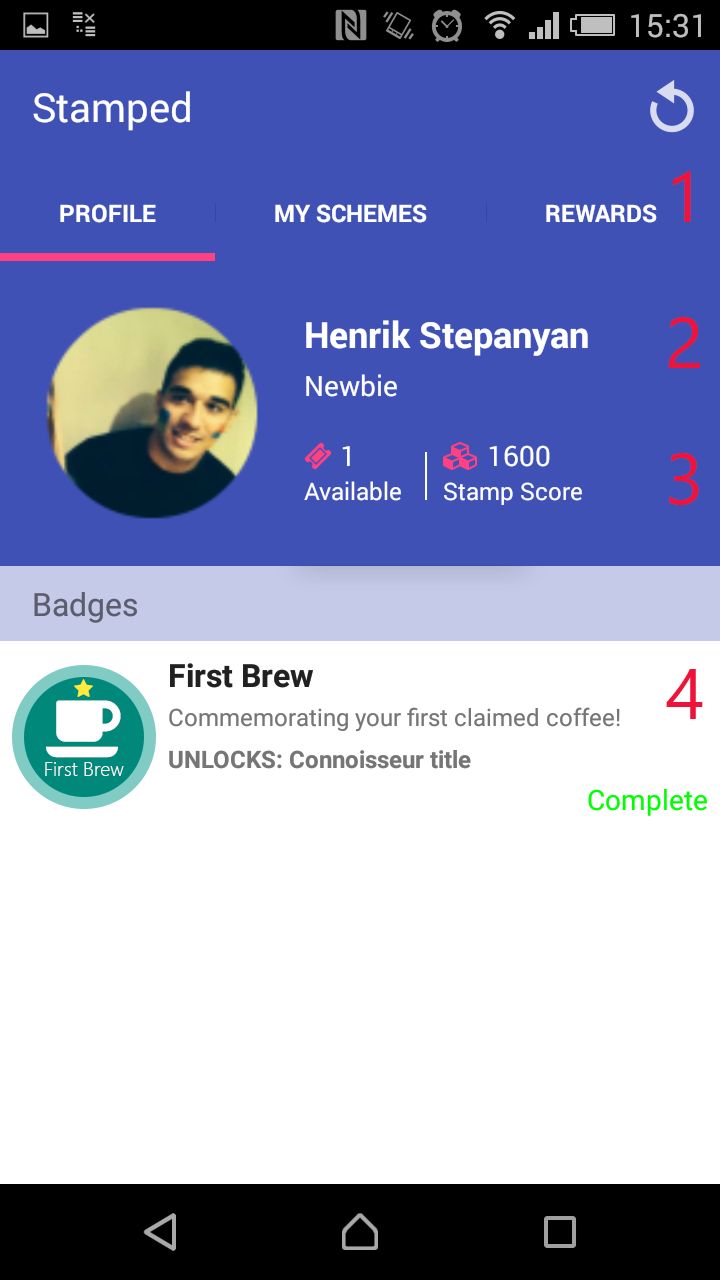
\includegraphics[width=0.275\textwidth]{img/moremock2.png}
   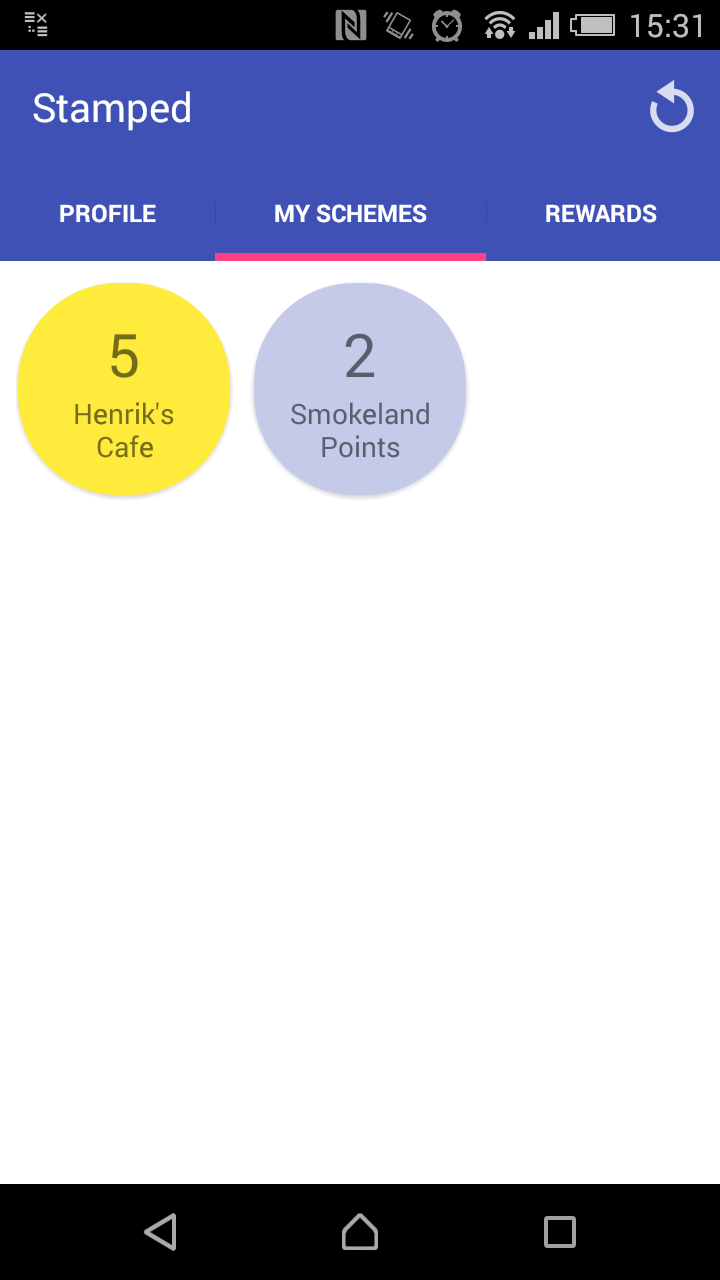
\includegraphics[width=0.275\textwidth]{img/finalmock.png}
    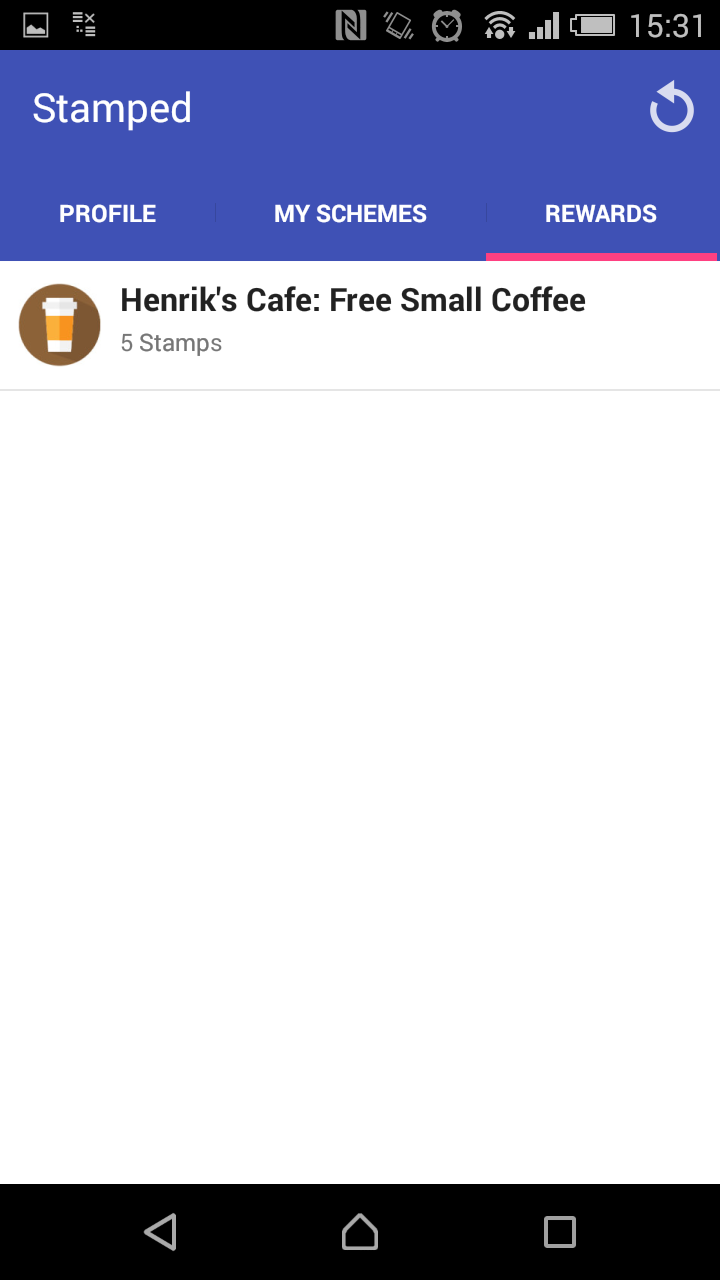
\includegraphics[width=0.275\textwidth]{img/moremock1.png}
     \caption{The final mockup of the Stampbook with a tabbed interface to be implemented}
     \label{fig:wireframe3}
\end{figure}

\begin{enumerate}
  \item A tabbed interface allows switching between different functional areas of an app, therefore making them very useful if functionality can be categorised. Profile, My Schemes and Rewards were chosen as the functional categories. An action button exists visibly on the top right to sync a the users profile (loyalty schemes/rewards etc.) with the server.
  \item The previous designs did not consider a user profile. The profile page aims to provide users a hub that presents them with their current account status. Customisability is also possible here, for instance the ability to add a profile picture, or to choose from a range of personal titles.
  \item Indicators are a key aspect of Nielsen's `visibility of system state' heuristic~\cite{jakob}. A count of available rewards notifies how many claimable rewards the user has; whereas stamp score is a gamification currency which could be used to claim exclusive rewards in the future. 
  \item A user profile is a prime location to display achieved user badges. This will be discussed in section\textit{(3.3.8 Incorporating Gamification/Persuassion)}
  \item Solutions we explored in the literature survey implemented loyalty schemes as lists. As a result, the `loyalty card' design from the previous iterations were transformed into bubbles within a grid. Businesses may be able to customize the background of the bubble with their own brand image. By pressing on the bubble, users are able to see the status of the scheme (Fig. \ref{fig:extrinsicmotivation}). Referencing previous feedback, a golden tint represents a loyalty scheme which has sufficient stamps to claim a reward.
  \item Further facilitating reward discovery, the dedicated rewards tab presents users with \textbf{all} available rewards they can afford with their stamps. This centralisation enforces a single convenient location to claim a reward. 
\end{enumerate}

\newpage
\subsection{Design Process - Loyalty Manager}
\subsubsection{Wire-Frame Mockups}
A similar design process was adopted for the loyalty manager. Wire-frames were developed on paper using the Material Design guidelines (Fig. \ref{fig:wireframem1}) 
\begin{figure}[H]
 \centering
  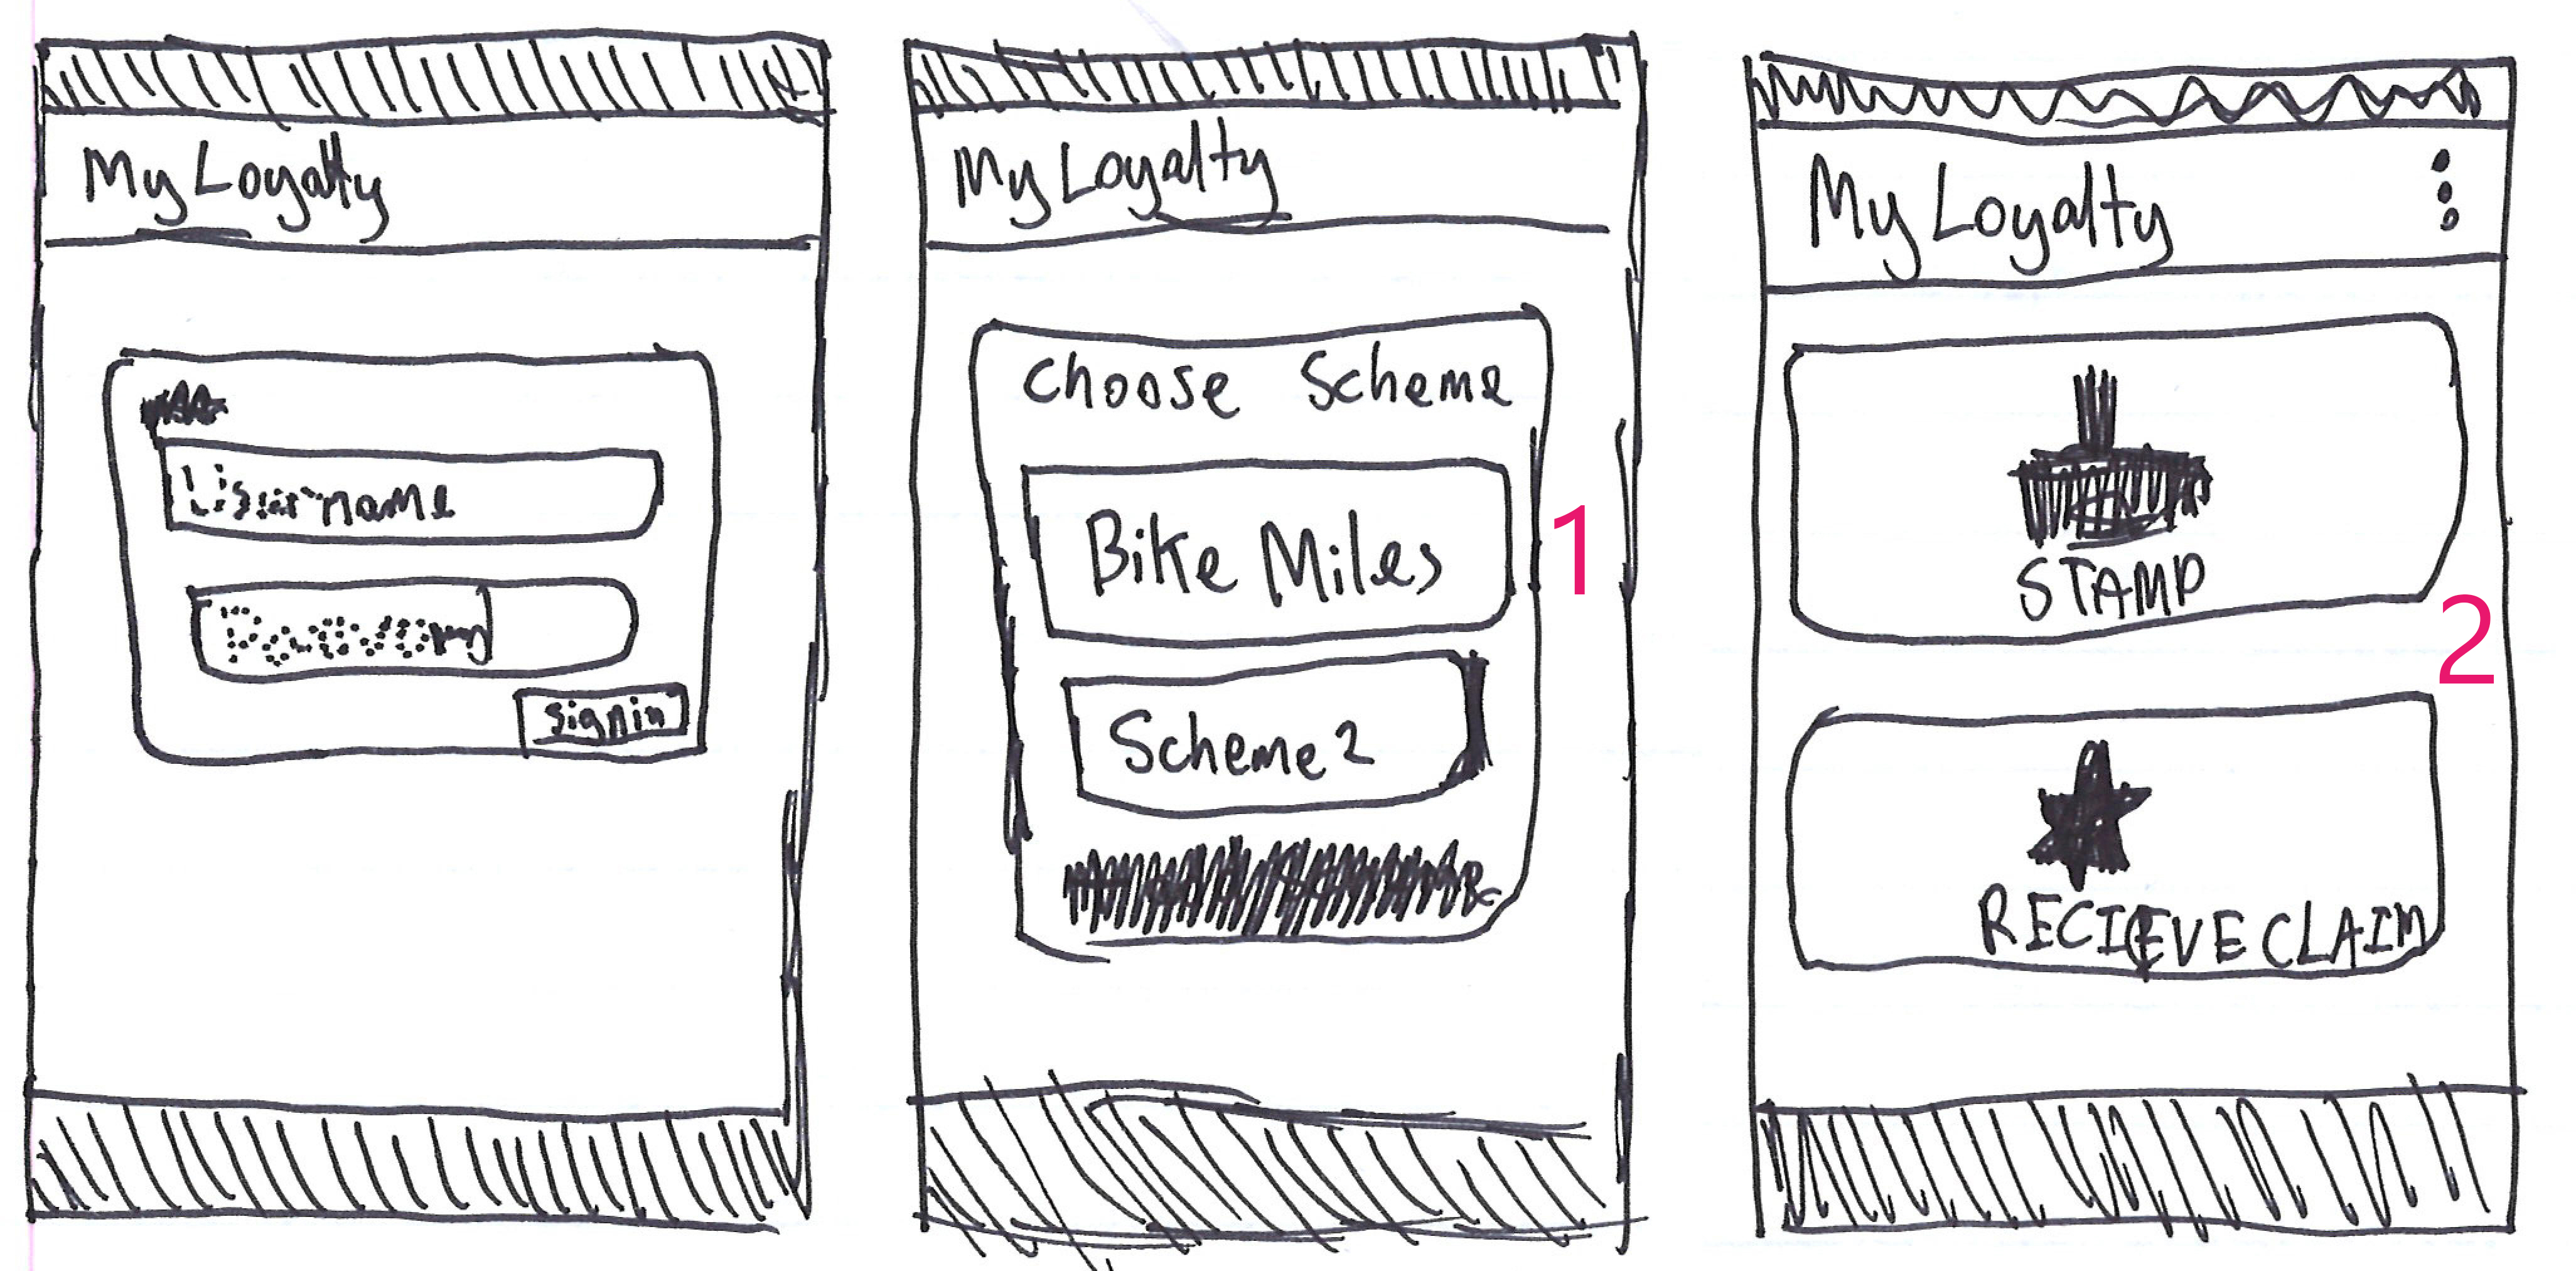
\includegraphics[width=0.9\textwidth]{img/Page2.jpg}
    \caption{The initial wireframe mockup for the Manager using the Material Design guidelines}
         \label{fig:wireframem1}
\end{figure}


\begin{enumerate}
  \item Users may manage more than loyalty scheme. As such, a menu is used in order to select the appropriate scheme.
  \item The stamp page is designed to be very simple with only two large accessible buttons. Pressing on either should enable the NFC chip in order to distribute a stamp or claim a user reward.
\end{enumerate}

\subsubsection{Feedback For Next Iteration}
\begin{itemize}
  \item \textit{``There should be a way to distribute multiple stamps''}
  \item \textit{``A log of recent transactions would be useful''}
  \item \textit{``The interface does not notify what loyalty scheme being stamped''}
\end{itemize}

As the functionality of this application is simpler than the Stampbook, feedback was easier to collect for the wire-frames. Suggestions, along with design patterns from the Stampbook were incorporated into the next iteration.

\subsubsection{Iteration 2 - Final Design}
A final design was developed by combining the aesthetic of the final Loyalty Stampbook prototype, with the suggestions from the previous wireframe  (Fig. \ref{fig:wireframem1}).
\begin{figure}[H]
 \centering
  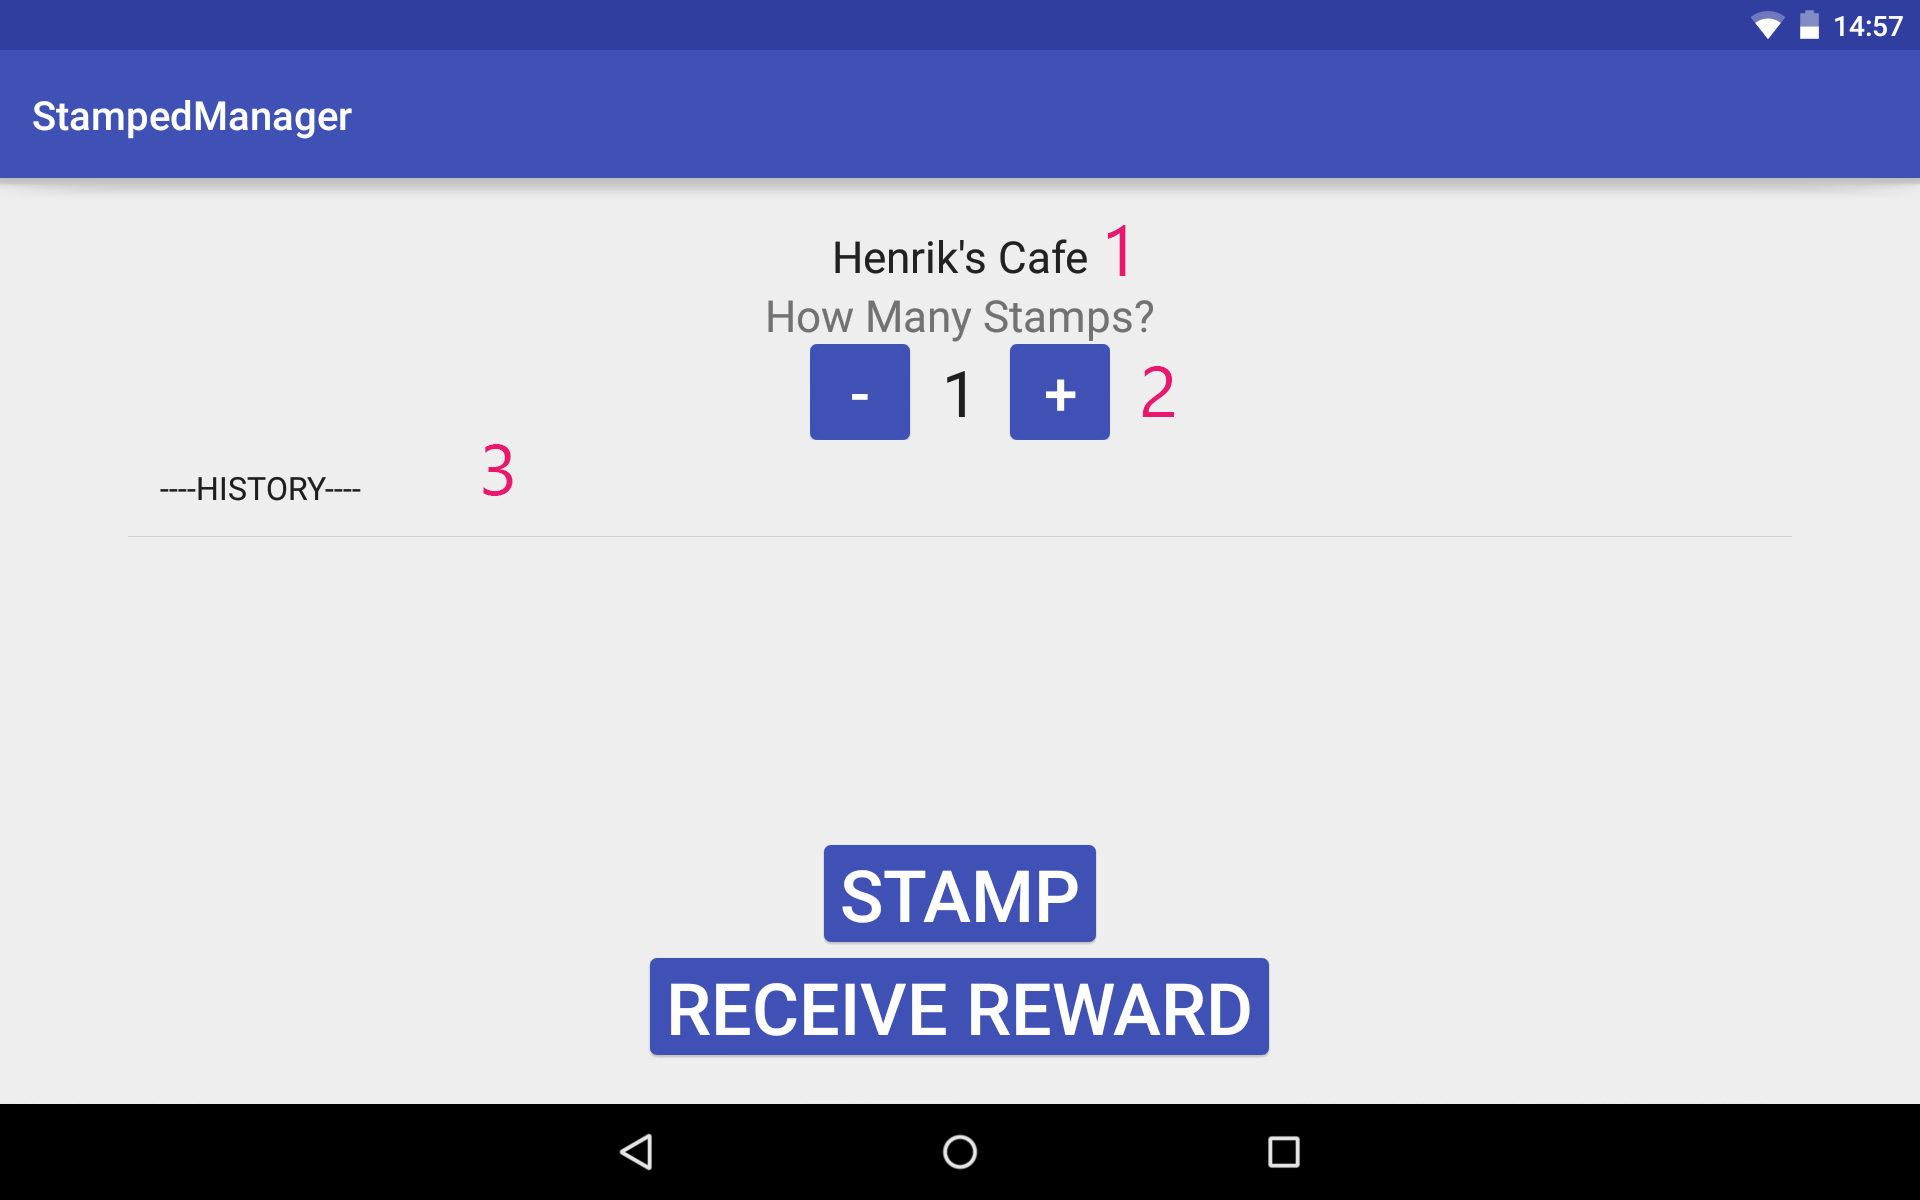
\includegraphics[width=0.494\textwidth]{img/readerfinalmock2.png}
   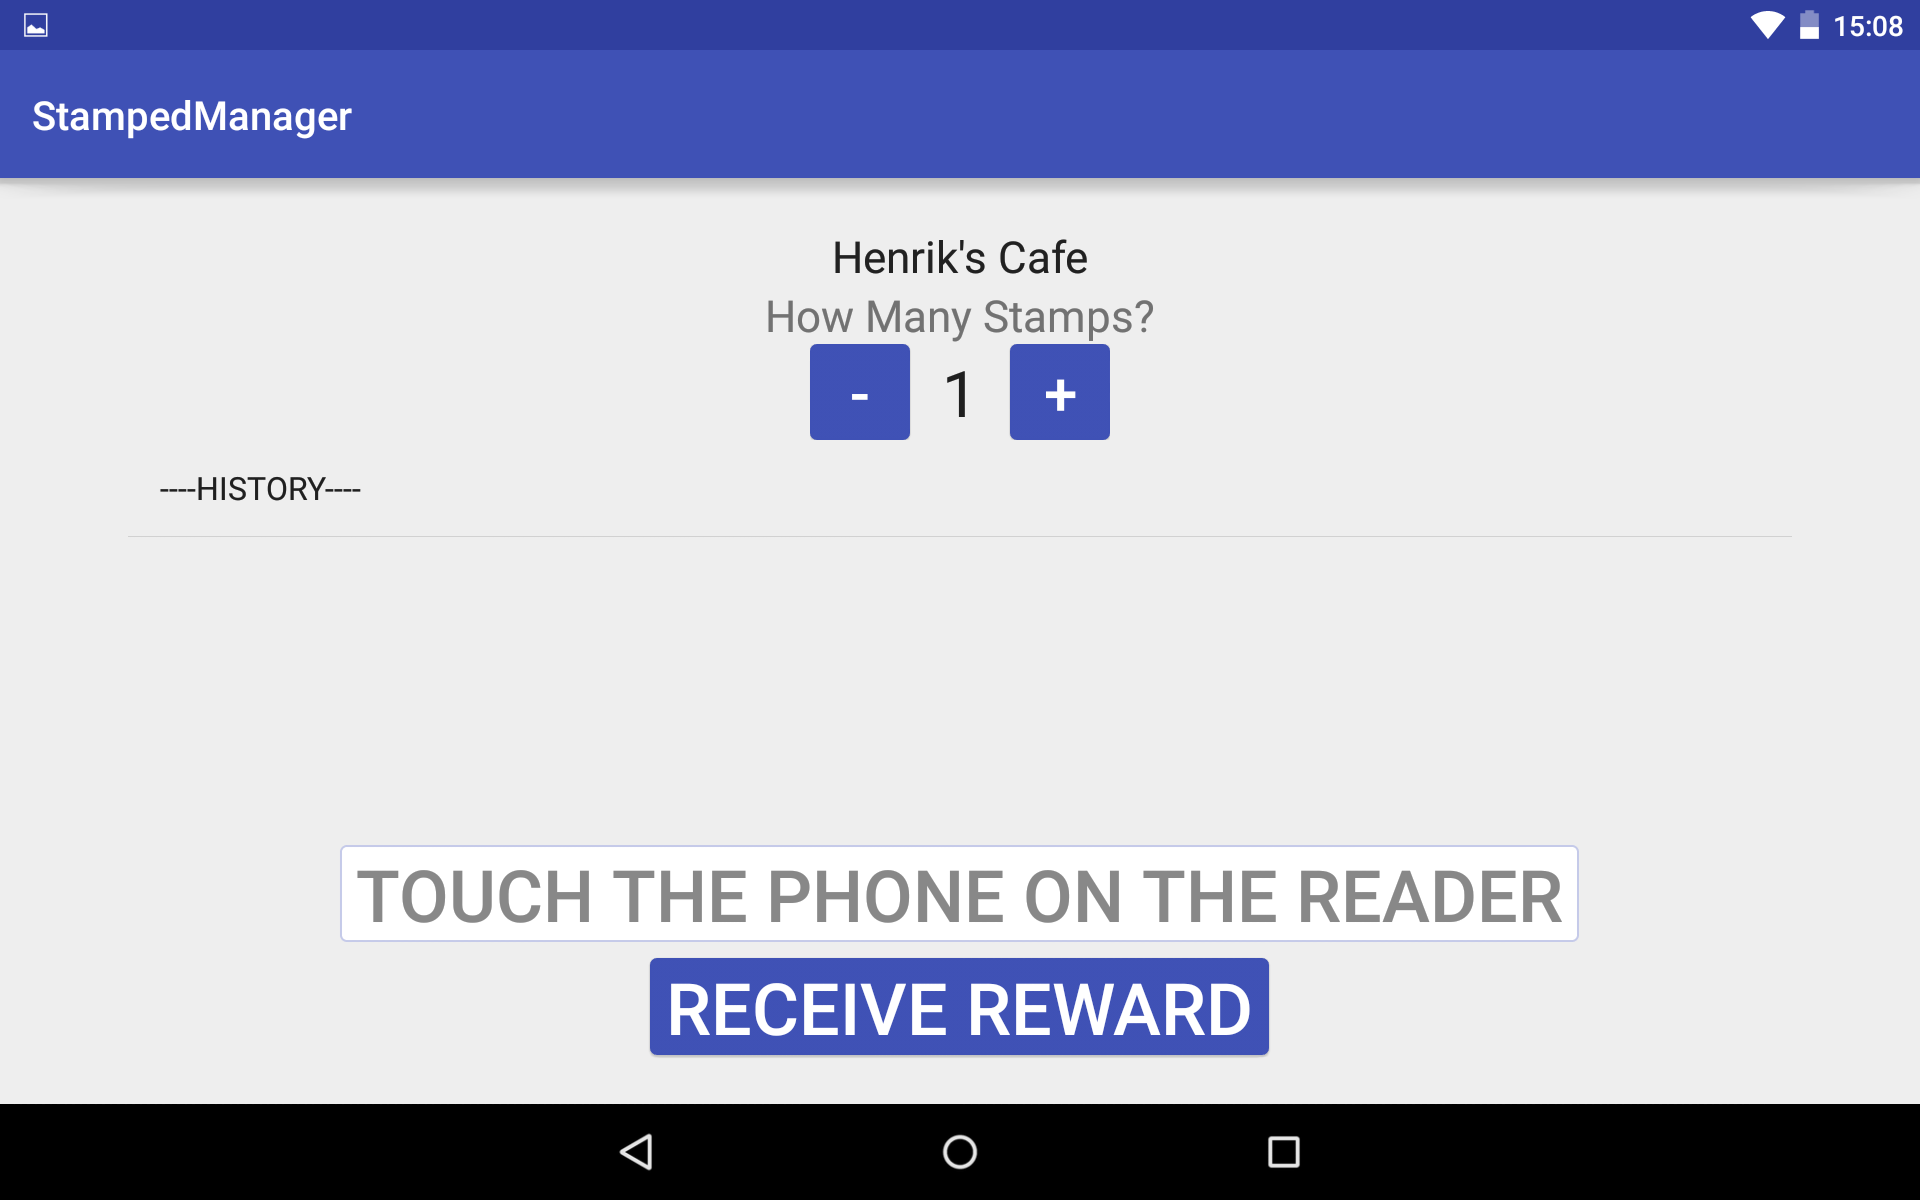
\includegraphics[width=0.494\textwidth]{img/readerfinalmock1.png}
     \caption{The final mockup of the Manager with the final aesthetic to be implemented}
     \label{fig:wireframem2}
\end{figure}

\begin{enumerate}
  \item A notifier of the current loyalty scheme, as suggested from previous feedback.
  \item A counter for the amount of stamps to distribute per tap. To facilitate ease of use, the number of stamps should reset back to one after every interaction. This will prevent any accidental `overstamping' previous customers if the business employee forgets to reset the value.
  \item The history provides a method of feedback to the employee. Upon all interactions, it should inform progress, successes and other key information regarding the loyalty schemes; however certain granularity had to be chosen.
\end{enumerate}

\newpage
\subsection{Design Process - Database Design}
\subsubsection{Entity-Relationship Diagram}
In section \ref{sec:databasepls} we identified the need for a database.
The design process was somewhat different than the applications as there was no user interface aspect involved. Initially, entities were identified for the schema - they were then normalised and translated into an Entity-Relationship Diagram (ERD)(Fig. \ref{fig:erd})~\cite{erd}.

\begin{figure}[H]
  \centering
    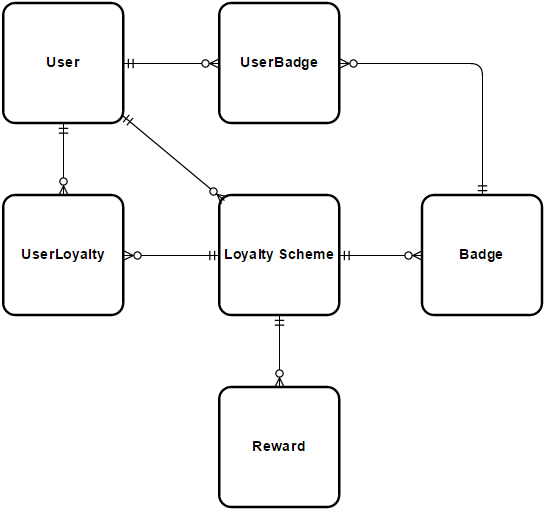
\includegraphics[width=0.8\textwidth]{img/erd.png}
      \caption{High-level Entity Relationship Diagram showing connections between different tables}
      \label{fig:erd}
\end{figure}

The following features were identified to be reflected as table attributes:
\begin{itemize}
  \item \textit{facilitation of the gamification platform}
  \item \textit{facilitation of scheme tracking/business intelligence}
\end{itemize}

\newpage
\subsubsection{Final Database Schema}
Building upon the initial ERD and incorporating the above features identified into the schema, a final database schema is proposed  (Fig. \ref{fig:finaldb}). 

\begin{figure}[H]
  \centering
    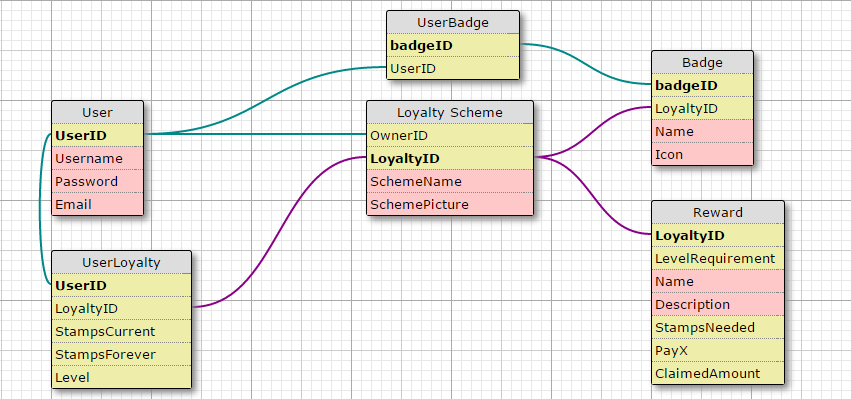
\includegraphics[width=0.8\textwidth]{img/architecture.png}
      \caption{Final database model to be implemented}
      \label{fig:finaldb}
\end{figure}

\subsubsection{Analysis of Final Schema}
In order to facilitate the gamification platform, we ensure that badges are independent from the loyalty schemes, affording the possible creation of unique badges by businesses. Moreover, the \emph{stampsForever} attribute of UserScheme can be used to monitor how often a user visits a business. Leaderboards as gamification are also possible from this field.

\emph{ClaimedAmount} from the Reward table, along with the aforementioned \emph{stampsForever} attribute can be used by businesses to track the popularity of their schemes. This allows them to monitor changes and adapt their schemes accordingly.

\newpage
\subsection{Incorporating Gamification/Persuassion}
\subsubsection{Extrinsic Motivation}
We previously defined the concept of `extrinsic motivation' as incentives where motives to enact the task are not related necessarily to that specific behaviour. These are commonly seen in loyalty cards - for instance users may not necessarily want to drink a coffee but want to complete their stamp card. Several solutions we explored in the literature review implemented digital stampcard-like solutions.

Similar to the systems we reviewed in chapter 2, a virtual stampcard metaphor was integrated into our design (Fig. \ref{fig:extrinsicmotivation}) as we felt it was familiar to users.
%affordances/stampbook + extrinsic motivvation + Nielsen match between world
\begin{figure}[H]
 \centering
  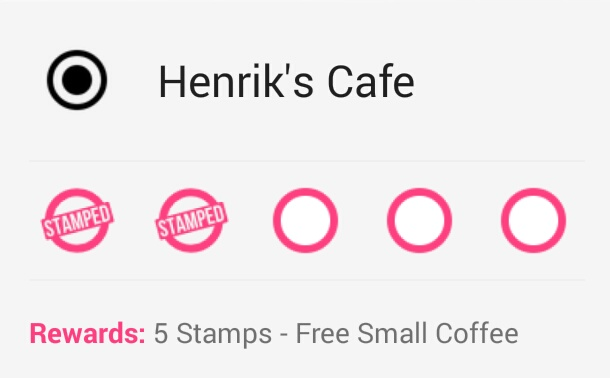
\includegraphics[width=0.40\textwidth]{img/stampcardprogress.jpg}
     \caption{The loyalty scheme view displaying: reward, current stamps and the amount of stamps left in order to gather the reward}
     \label{fig:extrinsicmotivation}
\end{figure}
\subsubsection{Badges}
Badges were identified earlier as a type of gamification tool. They were not only one of the more popular tools, but also the simplest to implement. As with real-life, badges are awarded upon achieving certain goals. As such, we introduce simple achievements into our system. Moreover, we require an incentive to collect badges -- therefore a title-system was added, allowing users to unlock certain and wear matching titles along with the achievement.

(Fig. \ref{fig:badge}) Shows how we integrated these principles into our design. The profile page makes an ideal home for collected badges.

\begin{figure}[H]
 \centering
  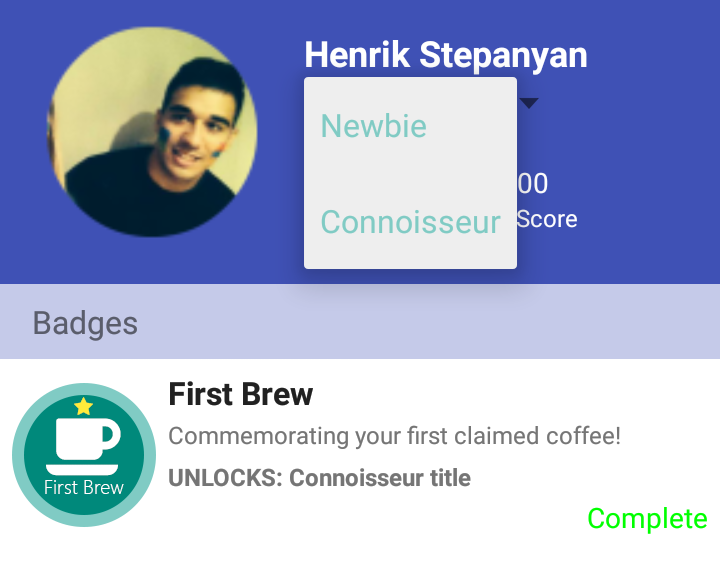
\includegraphics[width=0.40\textwidth]{img/badge.png}
     \caption{The badge view in the profile showing both the achievement and accompanied title earned by the user.}
     \label{fig:badge}
\end{figure}
\subsection{Naming The Systems}
In order to give the system a brand identity, it was named `Stamped' as it emphasises the software's focus on stamping. The `Loyalty Stampbook' is to be called \emph{Stamped}, whereas the `Loyalty Manager' is to be referred to as the \emph{Stamped Manager}. We hope that with a brand identity, users will be able to empathise and recognise the system better.
\subsection{Conclusion}
In this chapter we covered the requirements and design specification for our system `Stamped'. Some of the design challenges were outlined, along with the different iterations that eventually lead to the final designs. The next chapter will cover the issue of implementation.
